\documentclass[english, 11pt]{article}
\usepackage{../notes}

\newcommand{\thiscoursecode}{PHYS 234}
\newcommand{\thiscoursename}{Quantum Physics I}
\newcommand{\thisprof}{Dr. Robert Hill}
\newcommand{\me}{Liam Horne}
\newcommand{\thisterm}{Spring 2014}
\newcommand{\website}{LIHORNE.COM}

% Headers
\lhead{\thisterm}

%%%%% TITLE %%%%%
\newcommand{\notefront} {
\pagenumbering{roman}
\begin{center}

{\ttfamily \url{\website}} {\small}

\textbf{\Huge{\noun{\thiscoursecode}}}{\Huge \par}

{\Large{\noun{\thiscoursename}}}\\ \vspace{0.1in}

\vspace{0in}
\includegraphics[scale=0.5]{../logo.png}

  %\includegraphics[scale=0.1]{shield.png} \\
  {\noun \thisprof} \ $\bullet$ \ {\noun \thisterm} \ $\bullet$ \ {\noun {University of Waterloo}} \\

  \end{center}
  }

\newcommand{\bra}[1]{\langle #1 |}
\newcommand{\ket}[1]{| #1 \rangle}
\newcommand{\braket}[2]{\langle #1 | #2 \rangle}
\newcommand{\ba}{\bra{\alpha}}
\newcommand{\bb}{\bra{\beta}}
\newcommand{\bg}{\bra{\gamma}}
\newcommand{\ka}{| \alpha \rangle}
\newcommand{\kb}{| \beta \rangle}
\newcommand{\kg}{| \gamma \rangle}
\newcommand{\mtx}[1]{\left(\begin{matrix}#1\end{matrix}\right)}
\newcommand{\ebasis}{\ket{e_1}, \ket{e_2}, \ldots, \ket{e_n}}

%   ooooo      ooo   .oooooo.   ooooooooooooo oooooooooooo  .oooooo..o
%   `888b.     `8'  d8P'  `Y8b  8'   888   `8 `888'     `8 d8P'    `Y8
%    8 `88b.    8  888      888      888       888         Y88bo.
%    8   `88b.  8  888      888      888       888oooo8     `"Y8888o.
%    8     `88b.8  888      888      888       888    "         `"Y88b
%    8       `888  `88b    d88'      888       888       o oo     .d8P
%   o8o        `8   `Y8bood8P'      o888o     o888ooooood8 8""88888P'

\begin{document}

  % Notes fron
  \notefront
  % Table of Contents and List of Figures
  \tocandfigures
  % Abstract
  \doabstract{These notes are intended as a resource for myself; past, present, or future students of this course, and anyone interested in the material. The goal is to provide an end-to-end resource that covers all material discussed in the course displayed in an organized manner. If you spot any errors or would like to contribute, please contact me directly. \\}

  Robert Hill is a low temperature experimentalist, but this course will be mostly theoretical.
  \newline

   Albert Einstein once said, "Quantum mechanics is certainly imposing. But an inner voice tells me that it is not yet the realthing. The theory says a lot, but does not really bring us any closer to the secret of the 'old one'. I, at any rate, am convinced that He does not throw dice."
   \newline

   Richard Feynman said "I think I can safely say that nobody understand quantum mechanics."
   \newline

   So we're in for miserable experience with this course then? Well not really, there are some good reasons to study Quantum Physics:

   \begin{itemize}
     \item It's Extremely interesting!
     \begin{itemize}
        \item Physically
        \item Mathematically
        \item Philosophically
      \end{itemize}
      \item It is the science behind future technology!
      \item Waterloo is Quantum Valley!
   \end{itemize}

   \section{The Photoelectric and Compton Effects}

     \subsection{Historical Background}
       In classical physics we always observed things as behaving like waves or as particles. For example, there is

       \begin{itemize}
         \item Particle-like behaviour of radiation
         \item Wave-like behaviour of matter
         \item Wave-particle duality that combines the two
       \end{itemize}

       Let's explore the two sides of the coin. First, {\bf what is a particle?} Some words that describe it are {\textit point, localised, mass, solid} and similarly {\bf what is a wave?} It can be described with words like \textit{interference, oscillation, delocalised}, and \textit{medium}. One such thing that we have had trouble with describing is {\bf light}. Is it a wave or a particle?

     \subsection{Einstein's Theory of Photoelectric Effect}

       Radiant energy (light) is quantized into concentrated bundles (photons)

       \[ E = hf \]

       His Photoelectric Equation (1905) states that

       \[ K_{\mbox{max}} = hf - \omega_0 \]

     \subsection{Compton Effect}

       In the photoelectric effect, we treated light as being composed of individual light particles, called photons, that carry some energy. It then makes sense to think that the photons also have momentum.
       \newline

       Electromagnetic radiation is scattered by a target object. In classical theory, the charges in the target object will respond to the incoming wave and start to oscillate. All oscillating charges emit radiation at the frequency of oscillation, and this newly generated set of waves can also be detected at an angle θ with respect to the incoming wave. This classical model explains why the sky is blue and all that jazz. The scattering process itself, though, does not change the frequency of incoming and outgoing radiation.
       \newline

       However, an experimental problem occurred. In experiments with X-ray radiation on a graphene target, one observes that two separate frequencies at an angle $\theta$ result in different intensities. This effect is independent of the material, though intensities may vary.
       \newline

       \begin{defn}[Compton Shift]\label{compton_shift}
         \[ \Delta \lambda = \lambda_c (1 - \cos \theta) \]
       \end{defn}

       \begin{defn}[Compton wavelength]\label{compton_wavelength}
         \[ \lambda_c = \f{h}{m_0c} \]
       \end{defn}

       \begin{figure}[t]
         \centering
           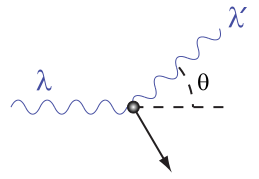
\includegraphics[width=0.35\textwidth]{compton_scattering.png}
         \caption{The Compton Effect. The scattered light has a different frequency; the frequency depends on the direction. A bigger deflection causes a bigger change in frequency.}
       \end{figure}

   \section{De Broglie Wavelength and the Davisson-Germer Experiement}

     We have shown that wave phenomena can exhibit particle features. We can rewrite the momentum instead as $p = \f{h}{\lambda}$ using a simple wave relationship. There is nothing in this reformed equation that has to do with light. This led to the following postulate.

     \subsection{The De Broglie Postulate (1924)}
       De Broglie's hypothesis was based on the grand symmetry of nature; if radiation has wave-particle duality, then so should matter.
       \begin{defn}[de Broglie Relation]\label{de_broglie_relation}
         \[ \lambda = \f{h}{p} \]
       \end{defn}

     \subsection{The Davisson-Germer Experiment}
       We must first understand the Bragg Grating; it is an optical filter that reflects particular wavelengths and transmits all others. Note that reflection, however, is common to both waves and particles.

     \subsection{Final Words}
       The observation of both phenomena in one and the same experiment leads us also to the concept of delocalization, which goes beyond the simple concept of "being extended", because single quantum objects seem to be able to simultaneously explore regions in space-time that cannot be explored by a single object in any classical way.

   \section{Linear Algebra Review}

     We're going to begin by reviewing some mathematics that will be needed in the course. This is a physics course so we're going to be a little loosey-goosey.

     \subsection{Vector Spaces}
        \begin{defn}[Vector Space]\label{vector_space}
          A {\bf vector space} consists of a set of vectors : ($|\alpha\rangle, |\beta\rangle, |\gamma\rangle, \ldots$) which is closed under vector addition and scalar multiplication.
        \end{defn}
        {\bf Vector Addition} produces another vector, that is
        \[ \ket{\alpha} + \ket{\beta} = \ket{\gamma}  \]
        it is also commutative
        \[ \ket{\alpha} + \ket{\beta} =  \ket{\beta}  + \ket{\alpha} \]
        and associative
        \[ \ket{\alpha} + (\ket{\beta} + \ket{\gamma}) =  (\ket{\alpha}+\ket{\beta} ) + \ket{\gamma} \]
        The null vector exists such that $\ket{\alpha} + \ket{0} = \ket{\alpha}$, and of course there is the inverse vector such that $\ket{\alpha} + \ket{-\alpha} = \ket{0}$.
        \newline

        {\bf Scalar Multiplication}: The product of a scalar with a vector is another vector ($a\ket{\alpha} = \ket{\gamma}$). Note that scalar multiplication is distributive with respect to vector addition
        \[ a(\ket{\alpha} + \ket{\beta}) = a\ket{\alpha} + a\ket{\beta} \]
        Scalar multiplication is distributive with respect to scalar addition too
        \[ (a + b)\ket{\alpha} = a\ket{\alpha} + b\ket{\alpha} \]
        and it is associative with respect to the product of scalars.
        \[ a(b \ket{\alpha}) = (ab)\ket{\alpha} \]
        then multiplication by zero and by $\pm 1$ has
        \[ 0\ket{\alpha} = \ket{0}, \ \ \ \ 1\ket{\alpha} = \ket{\alpha}, \ \ \ \ -1\ket{\alpha} = -\ket{\alpha} = \ket{-\alpha} \]
        \newline

        {\bf Linear Combinations of Vectors}: To generate a linear combination of vectors
        \[ \ket{\lambda} = a\ka + b\kb + c\kg \]
        \begin{itemize}
          \item[(I)] Any vector is linearly independent of a set of vectors if it cannot be written as a linear combination of them.
          \item[(II)] A set of vectors is linearly independent if each is linearly independent of the rest.
          \item[(III)] A colelction of vectors is said to {\bf span} the space if every vector can be written as a linear combination of them.
          \item[(IV)] A set of linearly independent vectors that span a space is called a {\bf basis}.
          \item[(V)] The number of vectors in the basis is called the {\bf dimension} of the space.\newline
        \end{itemize}

        {\bf Co-ordinate Representation}: With respect to a given basis, $\ket{e_1}, \ket{e_2}, \ket{e_3}, \hdots, \ket{e_n}$, any given vector $\ka = a_1 \ket{e_1} + a_2\ket{e_2} + \hdots + a_n \ket{e_n}$ is uniquely defined by the ordered $n$-tuple of its components.
        \[ \ka \iff \left(\begin{matrix}a_1 \\ a_2 \\ \vdots \\ a_n\end{matrix}\right) \]
        (the co-ordinate representation of $\ka$ with respect to the basis given by each $\ket{e_1}$.)

        Coordinates depend on the chosen basis. In basis 1 $\ka = a_x\ket{x} + a_y\ket{y} \iff \left(\begin{matrix}a_x \\ a_y \end{matrix}\right)$ and then in basis 2 we see $\ka = a_{x'}\ket{x'} + a_{y'}\ket{y'} \iff \mtx{a_{x'} \\ a_{y'}}$. \newline

        Addition of vectors by adding corresponding components (when in the same basis) works as you might expect, too:
        \[ \ket{\alpha} + \ket{\beta} \iff (a_1 + b_1, a_2 + b_2, \hdots, a_n + b_n \]

        Also, scalar multiplication works by multiplying the scalar in each component
        \[ c\ka \iff (ca_1, ca_2, ca_3, \ldots, ca_n) \]
        so of course,
        \[ \ket{0} = (0, 0, 0, \ldots, 0),  \ \ \ \ \ \ \  \ket{-\alpha} = (-a_1, -a_2, \ldots, -a_n) \]

        {\bf Inner Product}: For every vector, $\ka$, in a vector space there exists a dual vector $\bra{\alpha}$ in a corresponding dual vector space. Importantly, the dual vector to $c\ka$ is $C^*\bra{\alpha}$ where $*$ denotes complex conjugation. So the inner product of $\ka$ and $\kb$ is $\braket{\alpha}{\beta}$ which is a scalar (complex number), hence $\braket{\alpha}{\beta}$ is sometimes called {\bf scalar product}.

        \begin{itemize}
          \item[(I)] $\braket{\beta}{\alpha} = \braket{\alpha}{\beta}^*$
          \item[(II)] $\braket{\alpha}{\alpha} \geq 0$ (real and positive), so $\braket{\alpha}{\alpha} = 0$ if $\ka = \ket{0}$.
          \item[(III)] The norm of a vector $||\alpha|| = \sqrt{\braket{\alpha}{\alpha}}$ generalized "length" of a vector.
          \item[(IV)] Normalized $||\alpha|| = 1$.
          \item[(V)] Orthogonal if $\braket{\alpha}{\beta} = 0$, then $\ka$ is orthogonal to $\kb$.
          \item[(VI)] Orthogonal set $\braket{a_i}{a_j} = \delta_{ij} = \piecewise{1}{if $i = j$}{0}{if $i \not = j$}$
        \end{itemize}

        Consider the orthonormal basis $\ebasis$, and
        \[ \ka = a_1 \ket{e_1} + a_2 \ket{e_2} + \ldots + a_n \ket{e_n} \]
        \[ \kb = b_1 \ket{e_1} + b_2 \ket{e_2} + \ldots + b_n \ket{e_n} \]
        where we have the column vectors
        \[ \ka = \mtx{a_1 \\ a_2 \\ \vdots \\ a_n} \ \ \ \ \ \ \ \ \kb = \mtx{b_1 \\ b_2 \\ \vdots \\ b_n} \]
        then with dual vectors
        \[ \ka  = a_1^*\ket{e_1} + a_2^*\ket{e_2} + \ldots + a_n^*\ket{e_n} \]
        \[ \kb  = b_1^*\ket{e_1} + b_2^*\ket{e_2} + \ldots + b_n^*\ket{e_n} \]
        so that we have row vectors
        \[ \ka = (a_1^*, a_2^*, \ldots, a_n^*)  \ \ \ \ \ \ \ \ \kb = (b_1^*, b_2^*, \ldots,b_n^*) \]
        Now we can see that these results interact in a kind of cool way, check this out:
        \[ \braket{\alpha}{\beta} = (a_1^*, a_2^*, \ldots, a_n^*) \mtx{b_1 \\ b_2 \\ \vdots \\ b_n} = a_1^*b_1 + a_2^*b_2 + \ldots + a_n^* b_n \]
        which is a complex number. The components of the linear expansion are inner products too:
        \[ \ka = a_1\ket{e_1} + a_2\ket{e_2} + \ldots + a_n\ket{e_n} \]
        Consider also that
        \[ \braket{e_1}{\alpha} = \braket{e_1}{\left(a_1\ket{e_1} + a_2\ket{e_2} + \ldots + a_n\ket{e_n}\right)} = a_1\braket{e_1}{e_1} + a_2\braket{e_1}{e_2} + \ldots + a_n\braket{e_1}{e_n} = a_1\]



  \end{document}
